





\section{Final recommendations}
\label{section:final_recommendations_defect_control}
\subsection{The Vshaped graph and dependence on unit weight parameters}
\label{section:v_shaped_graph}
As we have shown several times in this thesis, the maximum order of accuracy of an interpolant depends on the value of the parameter $\alpha$ for the HB6 case and $\alpha$ and $\beta$ in the HB8 case. Furthermore, the accuracy also follows a V-shape as the interpolation error for sufficiently small $h$ reaches the round-off error. This is because the derivative of the interpolant uses a term in O($\frac{1}{h})$ where $h$ is the step-size. In this section we will look into how much these issues affect our interpolation. 

\paragraph{HB4}
In HB4, the error across several problems, across several sampling points, and at different step-sizes is as shown in Figure $\ref{fig:v_shape_across_problems_hb4}$. We note that this is without any parameters and at each h and each point $x$, we sampled at $x$ and $x + h$ to create the interpolant. The scheme suffers from an $O(\frac{1}{h})$ rounding off error inherently.
\begin{figure}[H]
\centering
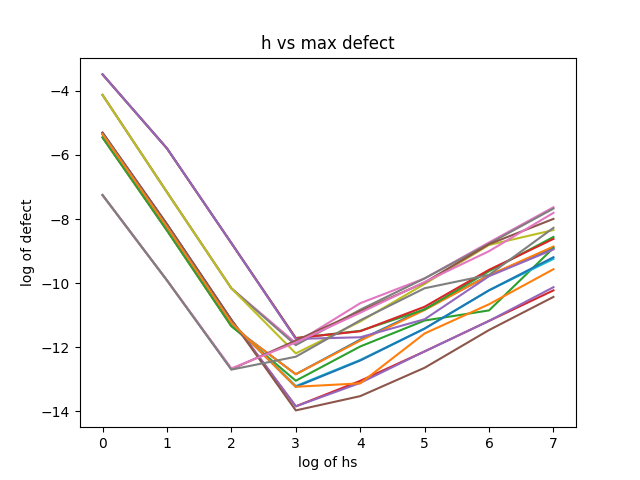
\includegraphics[width=0.7\linewidth]{./figures/v_shape_across_problems_hb4}
\caption{V-shape of HB4 across problems at several sampling points and with h.}
\label{fig:v_shape_across_problems_hb4}
\end{figure}

We note that there is a clear optimal $h$ at about $10^{-3}$ and that we are able to achieve a tolerance of  $10^{-14}$ with some problems and $10^{-12}$ with almost every other problem. This gives us hope that this scheme can be used at very sharp tolerances. In this section, we will try several techniques to improve the situation. 


\paragraph{HB6}
In HB6, the error across several problems, across several sampling points, and at different step-sizes is as shown in Figure $\ref{fig:v_shape_across_problems_hb6}$. We note that that the parameter $\alpha$ is constant at 1 throughout the whole process as we sample at the point, $x$ and the points $x+h$ and $x-h$. This is the ideal case as the interpolation error is thus minimised.

\begin{figure}[H]
\centering
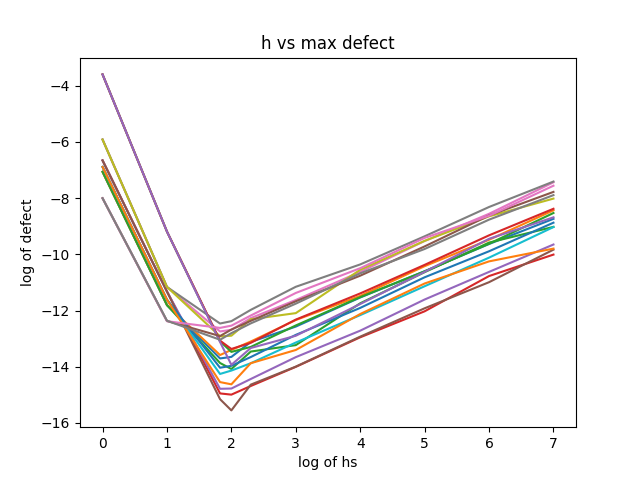
\includegraphics[width=0.7\linewidth]{./figures/v_shape_across_problems_hb6}
\caption{V-shape of HB6 across problems at several sampling points and with h.}
\label{fig:v_shape_across_problems_hb6}
\end{figure}

We note that $\alpha$ was kept at 1 in Figure $\ref{fig:v_shape_across_problems_hb6}$. To see how the parameter $\alpha$ reduces the accuracy as it deviates from 1, see Figure $\ref{fig:hb6_alpha_v_shape}$.

We can see that the optimal $h$ is at around $10^{-2}$. We note that in most cases we were able to reach an error of $10^{-14}$ but in some cases we were only able to solve at $10^{-12}$. 


\paragraph{HB8}
In HB8, the error across several problems, across several sampling points, and at different step-sizes is as shown in Figure $\ref{fig:v_shape_across_problems_hb8}$. We note that that both parameters $\alpha$ and $\beta$ were constant at 1 throughout the whole process as we sample at the point, $x$ and the points $x+h$, $x-h$ and $x-2h$. This is the ideal case as the interpolation error is thus minimised. 

\begin{figure}[H]
\centering
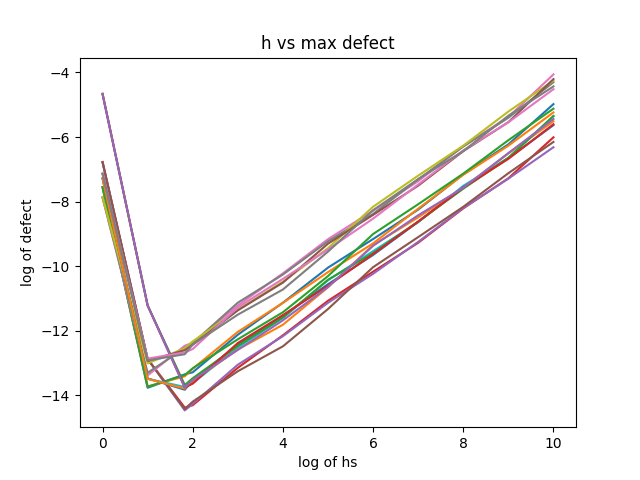
\includegraphics[width=0.7\linewidth]{./figures/v_shape_across_problems_hb8}
\caption{V-shape of HB8 across problems at several sampling points and with h.}
\label{fig:v_shape_across_problems_hb8}
\end{figure}

We note that both $\alpha$ and $\beta$ were kept at 1 in Figure $\ref{fig:v_shape_across_problems_hb8}$. To see how the parameters $\alpha$ and $\beta$ reduces the accuracy as it deviates from 1, see Figure $\ref{fig:hb8_second_scheme_alpha_beta_test}$.

We can see that the optimal $h$ is at around $10^{-1}$ and $10^{-2}$. We note that in most cases we were able to reach an error of $10^{-14}$ but in some cases we were only able to solve at $10^{-13}$. 

\subsection{Horner's and Barycentric interpolants to get to lower tolerances.}
\label{section:horner_bary_forms}
We note that up to this form, we have been using the monomial form of each of the cubic, quintic and septic polynomials that we have derived. In the previous section, we have shown how these were suffering from being eventually dominated by the rounding-off error as we use smaller and smaller step-sizes. One idea to deal with the loss of accuracy due to the interference from the rounding-off error is to use a different representation of the polynomials. 

One idea is to use the Horner's form of the polynomials. The Horner's form of a polynomial minimises the number of multiplications that need to be undertaken during the evaluation. It is faster and also a less prone to rounding-off errors since fewer arithmetic operations are involved.

Another idea is to use a Barycentric interpolant. At the time of the creation of the interpolant, if it is of order $n$ over the interval $[a, b]$, we can find $n$ Chebyshev points in the interval and then sample the interpolant at these $n$ points and then fit a Barycentric interpolant to these data points. A Barycentric interpolant using $n$ data points is of order $n$ and if such an interpolant is used to interpolate a polynomial of order $n$, it perfectly matches the polynomial that is, this process gives a different but exact representation of the original polynomial. The Chebyshev points are used to guarantee the minimum interpolation error.

We will use these two interpolation schemes to supplement the Hermite Birkhoff interpolants HB4, HB6 and HB8 at a few different sampling points at different problems and report on the improvements that they give.

\begin{figure}[H]
\centering
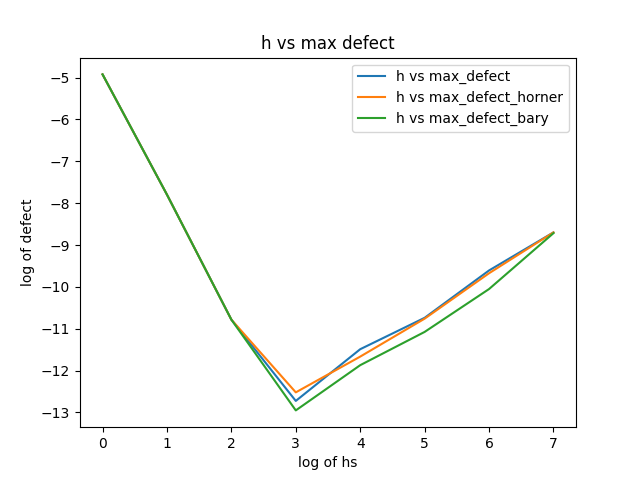
\includegraphics[width=0.7\linewidth]{./figures/typical_interp_horner_bary_hb4}
\caption{Typical plot of the HB4 interpolant monomial form vs the Horner form vs the Barycentric form.}
\label{fig:typical_interp_horner_bary_hb4}
\end{figure}

Figure $\ref{fig:typical_interp_horner_bary_hb4}$ shows a typical plot of HB4 in the monomial form alongside its Horner form and Barycentric interpolation forms. We can report that the Horner form almost always matches the accuracy of the interpolant but that the Barycentric form slightly improves the accuracy. The V-shape is inevitable as both forms either themselves suffer from $O(\frac{1}{h})$ rounding-off error or interpolate over an interpolant that suffers from such a rounding-off error.

\begin{figure}[H]
\centering
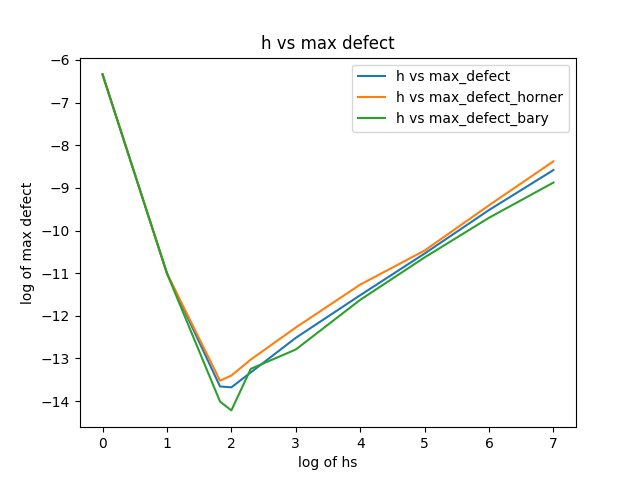
\includegraphics[width=0.7\linewidth]{./figures/typical_interp_horner_bary_hb6}
\caption{Typical plot of the HB6 interpolant monomial form vs the Horner form vs the Barycentric form.}
\label{fig:typical_interp_horner_bary_hb6}
\end{figure}

Figure $\ref{fig:typical_interp_horner_bary_hb6}$ shows a typical plot of HB6 in the monomial form alongside its Horner form and Barycentric interpolation forms. We note that the parameter $\alpha$ is kept at 1 in the above plot. We can report that the Horner form almost always matches the accuracy of the interpolant but that the Barycentric form slightly improves the accuracy. The V-shape is inevitable as both forms either themselves suffer from $O(\frac{1}{h})$ rounding-off error or interpolate over an interpolant that suffers from such a rounding-off error.

\begin{figure}[H]
\centering
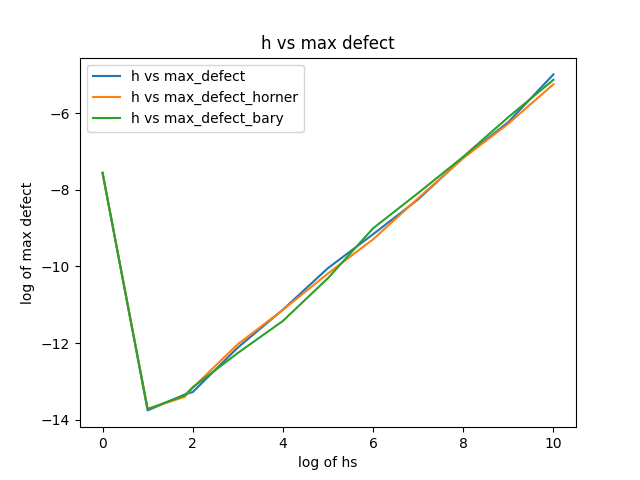
\includegraphics[width=0.7\linewidth]{./figures/typical_interp_horner_bary_hb8}
\caption{Typical plot of the HB8 interpolant monomial form vs the Horner form vs the Barycentric form.}
\label{fig:typical_interp_horner_bary_hb8}
\end{figure}

Figure $\ref{fig:typical_interp_horner_bary_hb8}$ shows the typical plot of HB6 in the monomial form alongside its Horner form and Barycentric interpolation forms. We note that the parameters $\alpha$ and $\beta$ are kept at 1 in the above plot. For the case of HB8, the use of the Horner method or even the Barycentric method does not improve the situation. The monomial form is as accurate as we can get. The V-shape is inevitable as both forms either themselves suffer from $O(\frac{1}{h})$ rounding-off error or interpolate over an interpolant that suffers from such a rounding-off error.

\label{section:defect_final_recommendations}
As we have noted before, all the interpolants have a V-shaped defect. We should note that experimentally, the trough for these V-shapes seem to be problem-independent. We thus used the optimal $h$ value, that is the $h$ value where the minimum maximum defect is found, as the initial $h$ value for each solver. We need this, especially in the variable parameter case, so that the first few steps are accepted. These optimal values are as follows. For HB4, the optimal $h$ value seems to be at about $10^{-3}$, for HB6, the optimal $h$ value seems to be at around $10^{-2}$ and for HB8, the optimal value seems to be at around $10^{-1}$ and $10^{-2}$. See Appendix $\ref{section:v_shaped_graph}$ for more details.

We also experimented with using representations of the polynomials other than the monomial form to reduce the effect of the rounding-off error. We can look to use the Barycentric or Horner form of the polynomials to improve the accuracy for example. (See Appendix $\ref{section:horner_bary_forms}$ for more details.)

Some recommendations for a final solver will be to start with the optimal h for the respective interpolant as the first step size so that the $\alpha$ and $\beta$ parameters do not get too large or too small for the first steps. In an ideal case, we would like to keep accepting steps at the start and allow the parameters to be close to 1 for as long as possible.

We should solve with a solver with variable $\alpha$ at the start and then if the solver fails too many step repeatedly, that is, the parameters get too far from 1, we should use the technique of forcing the parameters to be 1 and using the previous interpolants.

The first recommendation guarantees that the first few steps are taken at the minimum error possible and thus that they succeed. The second recommendation guarantees that if we meet a challenging behaviour at some point, we would be able to step through it with static parameters at the cost of additional function evaluations.

Another recommendation is to use different HB orders. An idea would be to use a lower order interpolant at coarser tolerances and use a higher order interpolant at sharper tolerances. 